\documentclass{article}
\usepackage[colorlinks, urlcolor=blue, linkcolor=red, citecolor=green]{hyperref}
\usepackage{fancyhdr} %设置页眉和页脚的
\usepackage{extramarks} %设置continue那玩意的
\usepackage{amsmath}
\usepackage{amsthm}
\usepackage{amsfonts}
\usepackage{tikz} %画线的
\usepackage[plain]{algorithm}
\usepackage{algpseudocode}
\usepackage{enumerate}
\usepackage{courier}
\usetikzlibrary{automata,positioning}

%表
\usepackage{booktabs}
\usepackage{multirow}
\usepackage{array}
\usepackage{caption}
\DeclareCaptionFont{heiti}{\heiti} %还可以定义其他的
\captionsetup{labelsep=space, font={small, bf}, skip=2pt} %space可以改成quad

%图
%*****************图片及其相关设置***************************
\usepackage{graphicx}
\graphicspath{{tupian/}}
\usepackage{subfigure}
% 导入tikz包
\usepackage{tikz}
\usetikzlibrary{math}

%*****************代码相关设置***************************
\usepackage{pythonhighlight}
%
% Basic Document Settings
%

\topmargin=-0.45in
\evensidemargin=0in
\oddsidemargin=0in
\textwidth=6.5in
\textheight=9.0in
\headsep=0.25in

\linespread{1.1}

\pagestyle{fancy}
\lhead{\hmwkAuthorName}
\chead{\hmwkClass: \hmwkTitle}
\rhead{\firstxmark}
\lfoot{\lastxmark}
\cfoot{\thepage}

\renewcommand\headrulewidth{0.4pt}
\renewcommand\footrulewidth{0.4pt}

\setlength\parindent{0pt}

%
% Create Problem Sections
%

\newcommand{\enterProblemHeader}[1]{
    \nobreak\extramarks{}{Problem \arabic{#1} continued on next page\ldots}\nobreak{}
    \nobreak\extramarks{Problem \arabic{#1} (continued)}{Problem \arabic{#1} continued on next page\ldots}\nobreak{}
}

\newcommand{\exitProblemHeader}[1]{
    \nobreak\extramarks{Problem \arabic{#1} (continued)}{Problem \arabic{#1} continued on next page\ldots}\nobreak{}
    \stepcounter{#1}
    \nobreak\extramarks{Problem \arabic{#1}}{}\nobreak{}
}

\setcounter{secnumdepth}{0}
\newcounter{partCounter}
\newcounter{homeworkProblemCounter}
\setcounter{homeworkProblemCounter}{1}
\nobreak\extramarks{Problem \arabic{homeworkProblemCounter}}{}\nobreak{}

\newenvironment{homeworkProblem}{
    \section{Problem \arabic{homeworkProblemCounter}}
    \setcounter{partCounter}{1}
    \enterProblemHeader{homeworkProblemCounter}
}{
    \exitProblemHeader{homeworkProblemCounter}
}

%
% Homework Details
%   - Title
%   - Due date
%   - Class
%   - Section/Time
%   - Instructor
%   - Author
%

\newcommand{\hmwkTitle}{Homework\ \#2}
\newcommand{\hmwkDueDate}{April 28, 2021}
\newcommand{\hmwkClass}{Deep Learning}
\newcommand{\hmwkClassTime}{}
\newcommand{\hmwkClassInstructor}{Professor Zhen Li}
\newcommand{\hmwkAuthorName}{Peng Deng}
\newcommand{\hmwkAuthorSchool}{School of Data Science}
\newcommand{\hmwkAuthorNumber}{Sno.220041042}
%
% Title Page
%

\title{
    \vspace{2in}
    \textmd{\textbf{\hmwkClass:\ \hmwkTitle}}\\
    \normalsize\vspace{0.1in}\small{Due\ on\ \hmwkDueDate}\\
    \vspace{0.1in}\large{\textit{\hmwkClassInstructor\ \hmwkClassTime}}
    \vspace{3in}
}

\author{\textbf{\hmwkAuthorName}}


\date{}

\renewcommand{\part}[1]{\textbf{\large Part \Alph{partCounter}}\stepcounter{partCounter}\\}

%
% Various Helper Commands
%

% Useful for algorithms
\newcommand{\alg}[1]{\textsc{\bfseries \footnotesize #1}}
\usepackage[algo2e,vlined,ruled]{algorithm2e}

% For derivatives
\newcommand{\deriv}[1]{\frac{\mathrm{d}}{\mathrm{d}x} (#1)}

% For partial derivatives
\newcommand{\pderiv}[2]{\frac{\partial}{\partial #1} (#2)}

% Integral dx
\newcommand{\dx}{\mathrm{d}x}

% Alias for the Solution section header
\newcommand{\solution}{\textbf{\large Solution}}

% Probability commands: Expectation, Variance, Covariance, Bias
\newcommand{\E}{\mathrm{E}}
\newcommand{\Var}{\mathrm{Var}}
\newcommand{\Cov}{\mathrm{Cov}}
\newcommand{\Bias}{\mathrm{Bias}}
\begin{document}

\maketitle
\thispagestyle{empty}

\newpage
\setcounter{page}{1}

\begin{homeworkProblem}
Equivariance is an appealing property when design neural network operations. It means that transforming the input image (e.g., translation) will also transform the output feature maps similarly after certain operations.

\vspace{4pt}
Formally, denote the image coordinate by $x \in \mathbb{Z}^{2}$, and the pixel values at each coordinate by a function $f: \mathbb{Z}^{2} \rightarrow \mathbb{Z}^{K}$, where $K$ is the number of image channels. A convolution filter can also be formulated as a function $w: \mathbb{Z}^{2} \rightarrow \mathbb{Z}^{K}$. Note that $f$ and $w$ are zero outside the image and filter kernel region, respectively. The convolution operation (correlation indeed for simplicity) is thus defined by
\begin{equation}
    [f * w](x)=\sum_{\mathbf{y} \in \mathbb{Z}^{2}} \sum_{k=1}^{K} f_{k}(y) w_{k}(y-x) .
\end{equation}
\begin{enumerate}[(a).]
    \item Let $L_{\mathrm{t}}$ be the translation $x \rightarrow x+t$ on the image or feature map, i.e.,
    $\left[L_{\mathrm{t}} f\right](x)=f(x-t)$. Prove that convolution has equivariance to translation:
    $$
    \left[\left[L_{\mathrm{t}} f\right] * w\right](x)=\left[L_{\mathrm{t}}[f * w]\right](x)
    $$
    which means that first translating the input image then doing the convolution is equivalent to first convolving with the image and then translating the output feature map. (Hints: Use the formula (1) for the proof.)    
    \item Let $L_{\mathbf{R}}$ be the $90^{\circ}$ -rotation on the image or feature map, where
    $$
    \mathbf{R}=\left[\begin{array}{cc}
    \cos (\pi / 2) & -\sin (\pi / 2) \\
    \sin (\pi / 2) & \cos (\pi / 2)
    \end{array}\right]
    $$
    then $\left[L_{\mathrm{R}} f\right](x)=f\left(\mathbf{R}^{-1} x\right)$. However, convolution is not equivariant to rotations,
    i.e., $\left[L_{\mathrm{R}} f\right] * w \neq L_{\mathrm{R}}[f * w]$, which is illustrated by Figure \ref{figp1} $((\mathrm{a})$ is not equivalent
    to
    (b) rotated by $90^{\circ}$ ). In order to establish the equivalence, the filter also needs to be rotated (i.e. (b) is equivalent to (c) in Figure \ref{figp1}). Prove that:
    $$
    \left[\left[L_{\mathrm{R}} f\right] * w\right](x)=L_{\mathbf{R}}\left[f *\left[L_{\mathbf{R}^{-1}} w\right]\right](x)
    $$
    (Hints: Use the formula (1) for the proof.)
\end{enumerate}


To make convolution equivariant to rotations, we need to extend the definition of convolution and transformation. Recall a group $(G, \otimes)$ in algebra is a set $G$, together with an binary operation
$\otimes$, which satisfies four requirements:

\qquad \textbf{Closure} \quad $a \otimes b \in G, \forall a, b \in G$

\qquad \textbf{Associativity}\quad $(a \otimes b) \otimes c=a \otimes(b \otimes c), \forall a, b, c \in G$ .

\qquad \textbf{Identity element} \quad  There exists a unique $e \in G, e \otimes a=a \otimes e=a, \forall a \in G$.

\qquad \textbf{Inverse element} \quad $\forall a \in G, \exists a^{-1} \in G, a \otimes a^{-1}=a^{-1} \otimes a=e$.

We can formulate $90^{\circ}$ -rotation and translation by a group $(G, \otimes)$ consisting of
$$
g(r, u, v)=\left[\begin{array}{ccc}
\cos (r \pi / 2) & -\sin (r \pi / 2) & u \\
\sin (r \pi / 2) & \cos (r \pi / 2) & v \\
0 & 0 & 1
\end{array}\right]
$$
where $r \in\{0,1,2,3\}$ and $(u, v) \in \mathbb{Z}^{2} . G=\{g\}$ and $\otimes$ is matrix multiplication. Translation is a
special case of $G$ when $r=0$ (i.e., $g(0, u, v))$ and rotation is a special case of $G$ when
$u=v=0$ (i.e., $g(r, 0,0))$.

\vspace{4pt}
A key concept is to extend the definition of both the feature $f$ and the filter $w$ to $G$. Imagine
the feature map is duplicated four times with rotation of $0^{\circ}, 90^{\circ}, 180^{\circ}$, and $270^{\circ}$. Then $f(g)$ is the feature values at particular rotated pixel coordinate, and the convolution operation becomes
$$
[f * w](g)=\sum_{\mathbf{h} \in G} \sum_{k=1}^{K} f_{k}(\mathbf{h}) w_{k}\left(g^{-1} \mathbf{h}\right) .
$$
A rotation-translation $u \in G$ on the feature map is thus $\left[L_{u} f\right](g)=f\left(u^{-1} g\right)$. Prove that under such extensions, the convolution is equivariant to rotation-translation:
$$
\left[\left[L_{u} f\right] * w\right](g)=L_{u}[f * w](g)
$$
\begin{enumerate}[a.]
    \setcounter{enumi}{2} 
    \item  Briefly explain how to implement this group convolution with traditional convolution and by rotating the feature map or filter. (Hints: Please read the paper "Group Equivariant Convolutional Networks").
\end{enumerate}
\begin{figure}[!htbp]
    \centering
    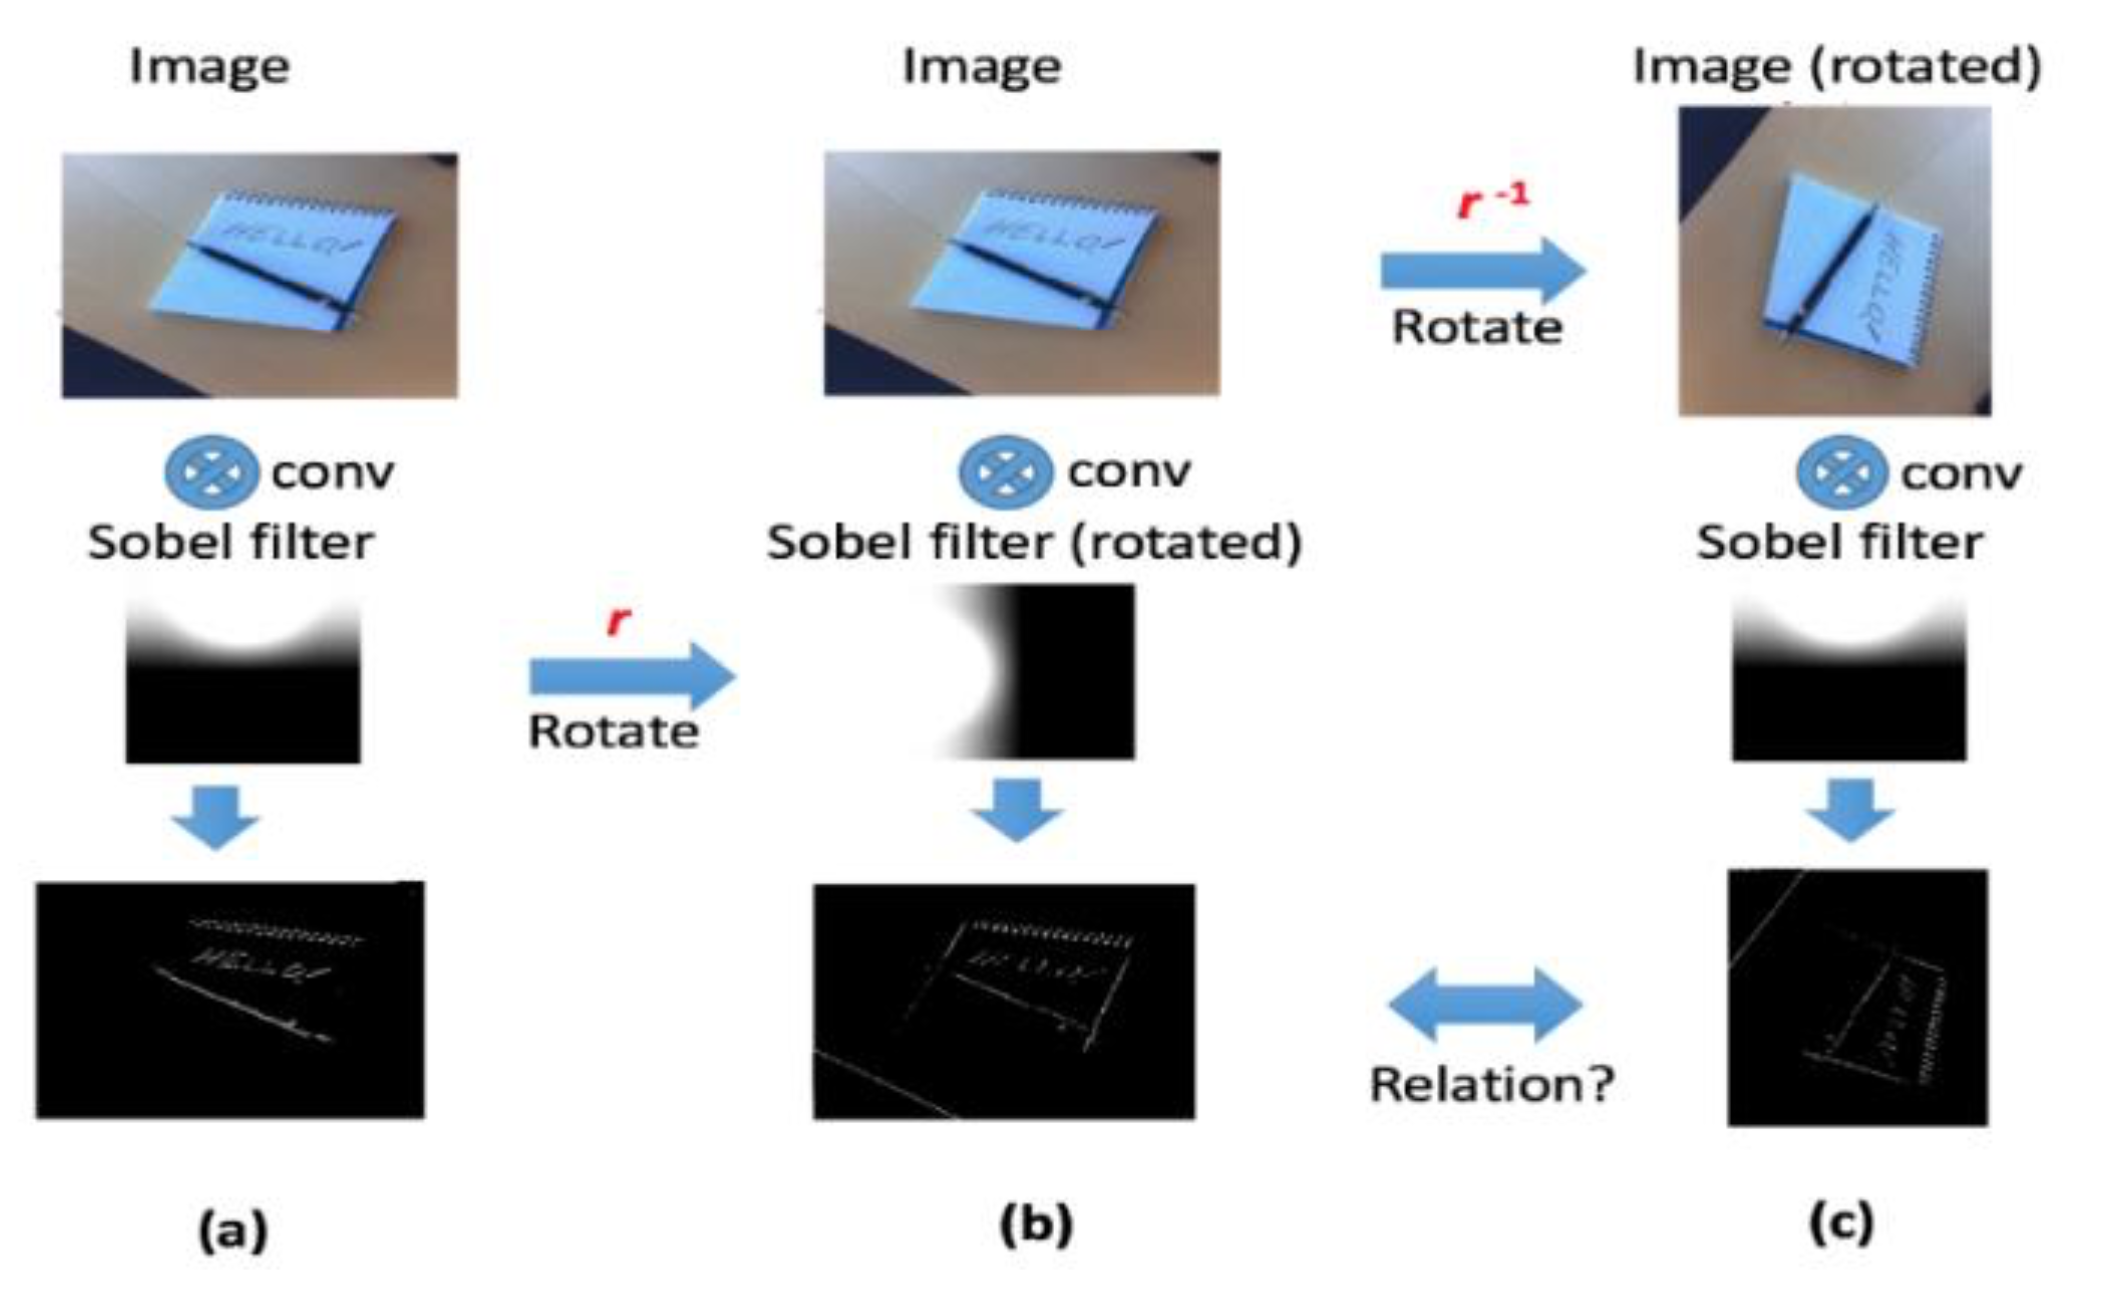
\includegraphics[width=0.6\linewidth]{images/p1.png}
    \caption{Equivariance relationship between convolution and rotation. (a) An image is convolved with a Sobel filer to detect horizontal edges. (b) The filter is rotated counterclockwise and then convolves the original image. (c) The image is first rotated clockwise, then it is convolved with the filter.}
    \label{figp1}
\end{figure}

\vspace{4pt}
\textbf{\large{Solution}}

\vspace{4pt}
\textbf{Subproblem(a)}

\begin{equation}
    \begin{split}
        \left[\left[L_{\mathbf{t}} f\right] * w\right](\boldsymbol{x}) &=\sum_{\boldsymbol{y} \in \mathbb{Z}^{2}} \sum_{k=1}^{K}\left[L_{\mathbf{t}} f\right]_{k}(\boldsymbol{y}) w_{k}(\boldsymbol{y}-\boldsymbol{x}) \\ 
            &=\sum_{\boldsymbol{y} \in \mathbb{Z}^{2}} \sum_{k=1}^{K} f_{k}(\boldsymbol{y}-\mathbf{t}) w_{k}(\boldsymbol{y}-\boldsymbol{x}) \\ 
            &=\sum_{\boldsymbol{y} \in \mathbb{Z}^{2}} \sum_{k=1}^{K} f_{k}(\boldsymbol{y}) w_{k}(\boldsymbol{y}+\boldsymbol{t}-\boldsymbol{x}) \\ 
            &=\sum_{\boldsymbol{y} \in \mathbb{Z}^{2}} \sum_{k=1}^{K} f_{k}(\boldsymbol{y}) w_{k}(\boldsymbol{y}-(\boldsymbol{x}-\boldsymbol{t})) \\ 
            \left[L_{\mathbf{t}}[f * w]\right](\boldsymbol{x})&=[f * w](\boldsymbol{x}-\boldsymbol{t})\\
            &=\sum_{\boldsymbol{y} \in \mathbb{Z}^{2}} \sum_{k=1}^{K} f_{k}(\boldsymbol{y}) w_{k}(\boldsymbol{y}-(\boldsymbol{x}-\boldsymbol{t})) \\ 
    \end{split}
\end{equation}
Thus, we finished the proof.

\vspace{4pt}
\textbf{Subproblem(b)}
\begin{equation}
    \begin{split}
        \left[\left[L_{\mathbf{R}} f\right] * w\right](\mathbf{x}) &=\sum_{\boldsymbol{y} \in \mathbb{Z}^{2}} \sum_{k=1}^{K}\left[L_{\mathbf{R}} f\right]_{k}(\boldsymbol{y}) w_{k}(\boldsymbol{y}-\boldsymbol{x}) \\ 
        &=\sum_{\boldsymbol{y} \in \mathbb{Z}^{2}} \sum_{k=1}^{K} f_{k}\left(\mathbf{R}^{-1} \boldsymbol{y}\right) w_{k}(\boldsymbol{y}-\boldsymbol{x}) \\ 
        &=\sum_{\boldsymbol{y} \in \mathbb{Z}^{2}} \sum_{k=1}^{K} f_{k}(\boldsymbol{y}) w_{k}(\mathbf{R} \boldsymbol{y}-\boldsymbol{x}) \\ 
        &=\sum_{\boldsymbol{y} \in \mathbb{Z}^{2}} \sum_{k=1}^{K} f_{k}(\boldsymbol{y}) w_{k}\left(\mathbf{R}\left(\boldsymbol{y}-\mathbf{R}^{-1} \boldsymbol{x}\right)\right) \\ 
        &=\sum_{\boldsymbol{y} \in \mathbb{Z}^{2}} \sum_{k=1}^{K} f_{k}(\boldsymbol{y})\left(\left[L_{\mathbf{R}^{-1}} w\right]_{k}\left(\boldsymbol{y}-\mathbf{R}^{-1} \boldsymbol{x}\right)\right) \\ 
        L_{\mathbf{R}}\left[f *\left[L_{\mathbf{R}^{-1}} w\right]\right](\boldsymbol{x})&=\left[f *\left[L_{\mathbf{R}^{-1}} w\right]\right]\left(\mathbf{R}^{-1} \boldsymbol{x}\right)\\
        &=\sum_{\boldsymbol{y} \in \mathbb{Z}^{2}} \sum_{k=1}^{K} f_{k}(\boldsymbol{y})\left(\left[L_{\mathbf{R}^{-1}} w\right]_{k}\left(\boldsymbol{y}-\mathbf{R}^{-1} \boldsymbol{x}\right)\right) \\ 
    \end{split}
\end{equation}
Thus, we finished the proof.

\vspace{4pt}
\textbf{Subproblem(c)}
\begin{equation}
    \begin{split}
        \left[\left[L_{\mathbf{u}} f\right] * w\right](\mathbf{g}) &=\sum_{\mathbf{h} \in G} \sum_{k=1}^{K}\left[L_{\mathbf{u}} f\right]_{k}(\mathbf{h}) w_{k}\left(\mathbf{g}^{-1} \mathbf{h}\right) \\ 
        &=\sum_{\mathbf{h} \in G} \sum_{k=1}^{K} f_{k}\left(\mathbf{u}^{-1} \mathbf{h}\right) w_{k}\left(\mathbf{g}^{-1} \mathbf{h}\right) \\ 
        &=\sum_{\mathbf{h} \in G} \sum_{k=1}^{K} f_{k}(\mathbf{h}) w_{k}\left(\mathbf{g}^{-1} \mathbf{u h}\right) \\ 
        &=\sum_{\mathbf{h} \in G} \sum_{k=1}^{K} f_{k}(\mathbf{h}) w_{k}\left(\left(\mathbf{u}^{-1} \mathbf{g}\right)^{-1} \mathbf{h}\right) \\ 
        &=[f * w]\left(\mathbf{u}^{-1} \mathbf{g}\right)=\left[L_{\mathbf{u}}[f * w]\right](\mathbf{g})
    \end{split}
\end{equation}
Thus, we finished the proof.

\vspace{4pt}
To implement this group convolution, we just need to
\begin{enumerate}[(a)]
    \item duplicate and rotate the input image by $\left\{0^{\circ}, 90^{\circ}, 180^{\circ}, 270^{\circ}\right\}$, which leads to four times of input channels;
    \item duplicate and rotate the original filters by $\left\{0^{\circ}, 90^{\circ}, 180^{\circ}, 270^{\circ}\right\}$. 
\end{enumerate}
\end{homeworkProblem}

\begin{homeworkProblem}
A recurrent neural network is shown in Figure \ref{figp2}.
\begin{figure}[!htbp]
    \centering
    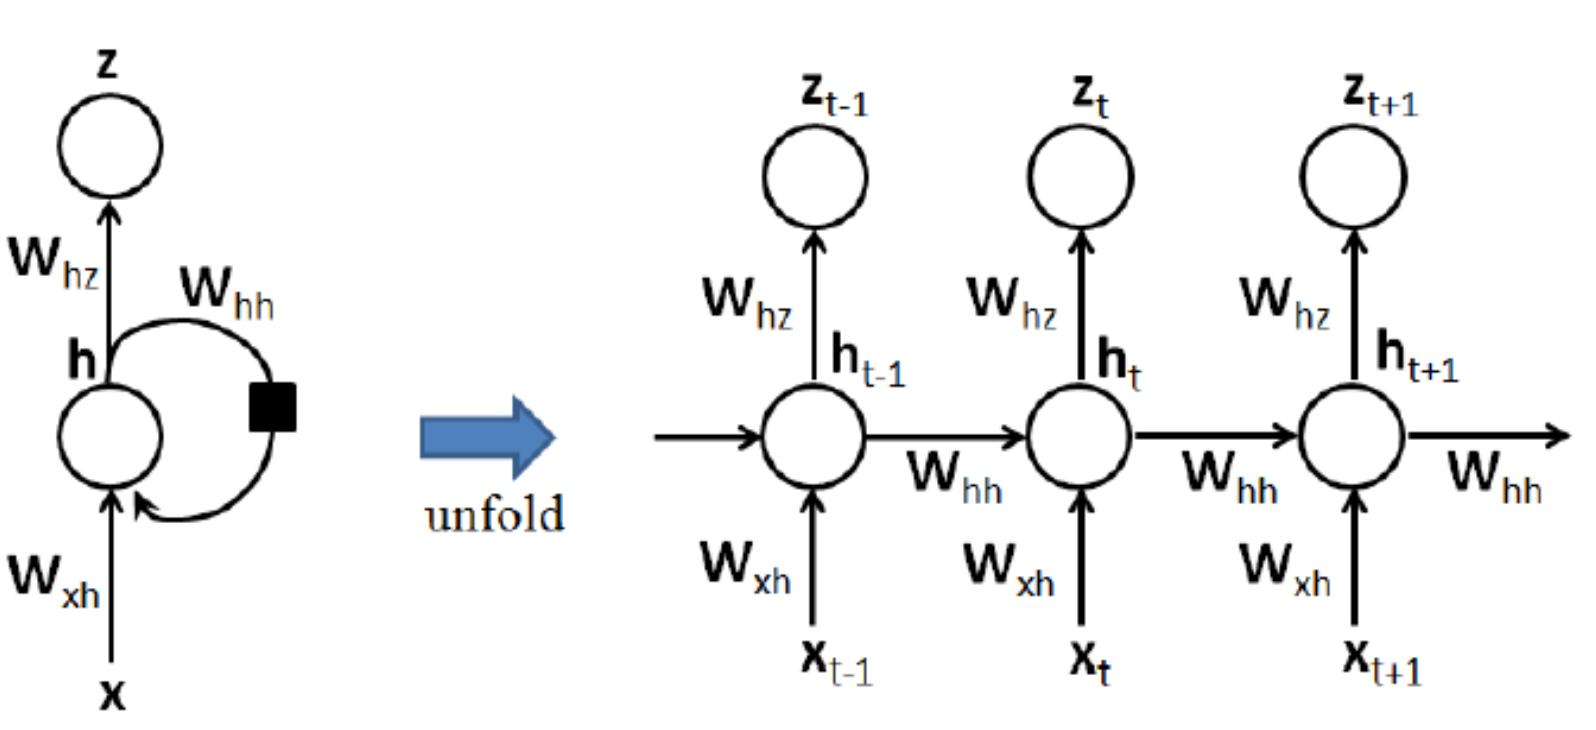
\includegraphics[width=0.6\linewidth]{images/p2.png}
    \caption{RNN fold and unfold structure.}
    \label{figp2}
\end{figure}

$$
\begin{array}{c}
h_{t}=\tanh \left(\mathbf{W}_{x h} x_{t}+\mathbf{W}_{h h} h_{t-1}+b_{h}\right) \\
z_{t}=\operatorname{softmax}\left(\mathbf{W}_{h z} h_{t}+b_{z}\right)
\end{array}
$$
The total loss for a given input/target sequence pair (x, y), measured in cross entropy
$$
L(x, y)=\sum_{t} L_{t}=\sum_{t}-\log z_{t, y_{t}}
$$
In the lecture, we provide the general idea of how to calculate the gradients $\frac{\partial L}{\partial W_{h z}}$ and $\frac{\partial L}{\partial W_{h h}}$. Please provide the details of the algorithms and equations, considering the mapping and cost functions provided above.

\vspace{4pt}
\textbf{\large{Solution}}

\vspace{4pt}
\textbf{Part (1)}

Let $\boldsymbol{u_t}=\boldsymbol{W}_{hz}\boldsymbol{h}_t+\boldsymbol{b}_z$, so $\boldsymbol{z}_t=\operatorname{softmax}\left(\boldsymbol{u}_t\right)$. Let $\boldsymbol{y}_t$ be the 
one-hot representation of label at time $t$. Then we have
\begin{equation}
    \begin{split}
        \frac{\partial L_t}{\partial \boldsymbol{u}_t}&=\frac{\partial L_t}{\partial \boldsymbol{z}_t}\cdot \frac{\partial \boldsymbol{z}_t}{\partial \boldsymbol{u}_t}=\boldsymbol{z}_t - \boldsymbol{y}_t\\
        \Longrightarrow\frac{\partial L_t}{\partial \boldsymbol{u}_{t,i}}&=\boldsymbol{z}_{t,i} - \boldsymbol{y}_{t,i}\\
    \end{split}
\end{equation}
Then, we can derive $\frac{\partial\boldsymbol{u}_{t,i}}{\partial\boldsymbol{W}_{hz,ij}}$ as follow
\begin{equation}
    \frac{\partial\boldsymbol{u}_{t,i}}{\partial\boldsymbol{W}_{hz,ij}}=\boldsymbol{h}_{t,j}
\end{equation}
Then, we can derive $\frac{\partial L_{t}}{\partial\boldsymbol{W}_{hz}}$
\begin{equation}
    \begin{split}
        \frac{\partial L_{t}}{\partial\boldsymbol{W}_{hz,ij}}&=\frac{\partial L_{t}}{\partial \boldsymbol{u}_{t,i}}\cdot\frac{\partial \boldsymbol{u}_{t,i}}{\partial\boldsymbol{W}_{hz,ij}}\\
        &=\left(\boldsymbol{z}_{t,i} - \boldsymbol{y}_{t,i}\right)\cdot\boldsymbol{h}_{t,j}\\
        \Longrightarrow \frac{\partial L_{t}}{\partial\boldsymbol{W}_{hz}}&=\left(\boldsymbol{z}_t-\boldsymbol{y}_t\right)\cdot \boldsymbol{h}_t^{\top}
    \end{split}
\end{equation}
Finally, we can derive $\frac{\partial L}{\partial\boldsymbol{W}_{hz}}$ as follow
\begin{equation}
    \begin{split}
        \frac{\partial L}{\partial\boldsymbol{W}_{hz}}&=\frac{\partial \sum_t L_t}{\partial\boldsymbol{W}_{hz}}\\
        &=\sum_t \frac{\partial L_t}{\partial\boldsymbol{W}_{hz}}\\
        &=\sum_t \left(\boldsymbol{z}_t-\boldsymbol{y}_t\right)\cdot \boldsymbol{h}_t^{\top}
    \end{split}
\end{equation}
\vspace{4pt}
\textbf{Part (2)}

Let $\boldsymbol{v}_t = \mathbf{W}_{x h} \boldsymbol{x}_{t}+\mathbf{W}_{h h} \boldsymbol{h}_{t-1}+\boldsymbol{b}_{h}$, then we have
\begin{equation}
    \label{eq8}
    \begin{split}
        \frac{\partial L}{\partial \boldsymbol{W}_{hh}}&=\sum_t \frac{\partial L}{\partial \boldsymbol{h}_{t}}\cdot\frac{\partial \boldsymbol{h}_{t}}{\partial \boldsymbol{W}_{hh}}\\
        \Longrightarrow \frac{\partial L}{\partial \boldsymbol{W}_{hh,ij}}&=\sum_t \frac{\partial L}{\partial \boldsymbol{h}_{t,i}}\cdot\frac{\partial \boldsymbol{h}_{t,i}}{\partial \boldsymbol{W}_{hh,ij}}\\
        &=\sum_t \frac{\partial L}{\partial \boldsymbol{h}_{t,i}}\cdot\frac{\partial \boldsymbol{h}_{t,i}}{\partial \boldsymbol{v}_{t,i}}\cdot\frac{\partial \boldsymbol{v}_{t,i}}{\partial \boldsymbol{W}_{hh,ij}}\\
        &=\sum_t \frac{\partial L}{\partial \boldsymbol{h}_{t,i}}\cdot\left(1-\boldsymbol{h}_{t,i}^2\right)\cdot\boldsymbol{h}_{t-1,j}\\
    \end{split}
\end{equation}
We can derive $\frac{\partial L}{\partial \boldsymbol{h}_{t}}$ as follow
\begin{equation}
    \label{eq9}
    \begin{split}
        \frac{\partial L}{\partial \boldsymbol{h}_{t}}&=\frac{\partial L}{\partial \boldsymbol{h}_{t+1}}\cdot\frac{\partial \boldsymbol{h}_{t+1}}{\partial \boldsymbol{h}_{t}}+\frac{\partial L}{\partial \boldsymbol{u}_{t}}\cdot\frac{\partial \boldsymbol{u}_{t}}{\partial \boldsymbol{h}_{t}}\\
        &=\frac{\partial L}{\partial \boldsymbol{h}_{t+1}}\cdot\frac{\partial \boldsymbol{h}_{t+1}}{\partial \boldsymbol{v}_{t+1}}\cdot \frac{\partial \boldsymbol{v}_{t+1}}{\partial \boldsymbol{h}_{t}}+\left(\boldsymbol{z}_t-\boldsymbol{y}_t\right)^{\top}\boldsymbol{W}_{hz}\\
        &=\frac{\partial L}{\partial \boldsymbol{h}_{t+1}}\cdot\operatorname{diag\left(1-\boldsymbol{h}_{t+1}^2\right)}\cdot \boldsymbol{W}_{hh}+\left(\boldsymbol{z}_t-\boldsymbol{y}_t\right)^{\top}\boldsymbol{W}_{hz}\\
    \end{split}
\end{equation}
The term $\frac{\partial L}{\partial \boldsymbol{h}_{t,i}}$ in equation \ref{eq8} can be derived from equation \ref{eq9}. Besides, the term is a recursive term.
\end{homeworkProblem}

\begin{homeworkProblem}
    Consider an episodic, deterministic chain MDP with $\mathrm{n}=7$ states assembled in a line.
The possible actions are $a \in\{-1,1\}$, and the transition function is deterministic such that
$s^{\prime}=s+a .$ Note that as an exception, taking $a=-1$ from $s=1$ keeps us in $s=1$, and taking $a=-1$ from $s=7$ keeps us in $s=7$.

We have a special goal state, $g=4$, such that taking any action from $g$ ends the episode with a reward of $r=0$. From all other states, any action incurs a reward of $r=-1$. We let discount factor $\gamma=1 / 3$.

\vspace{4pt}
The chain MDP is pictured in Figure \ref{figp3}, with the goal state $s_4$ shaded in.
\begin{figure}[H]
    \centering
    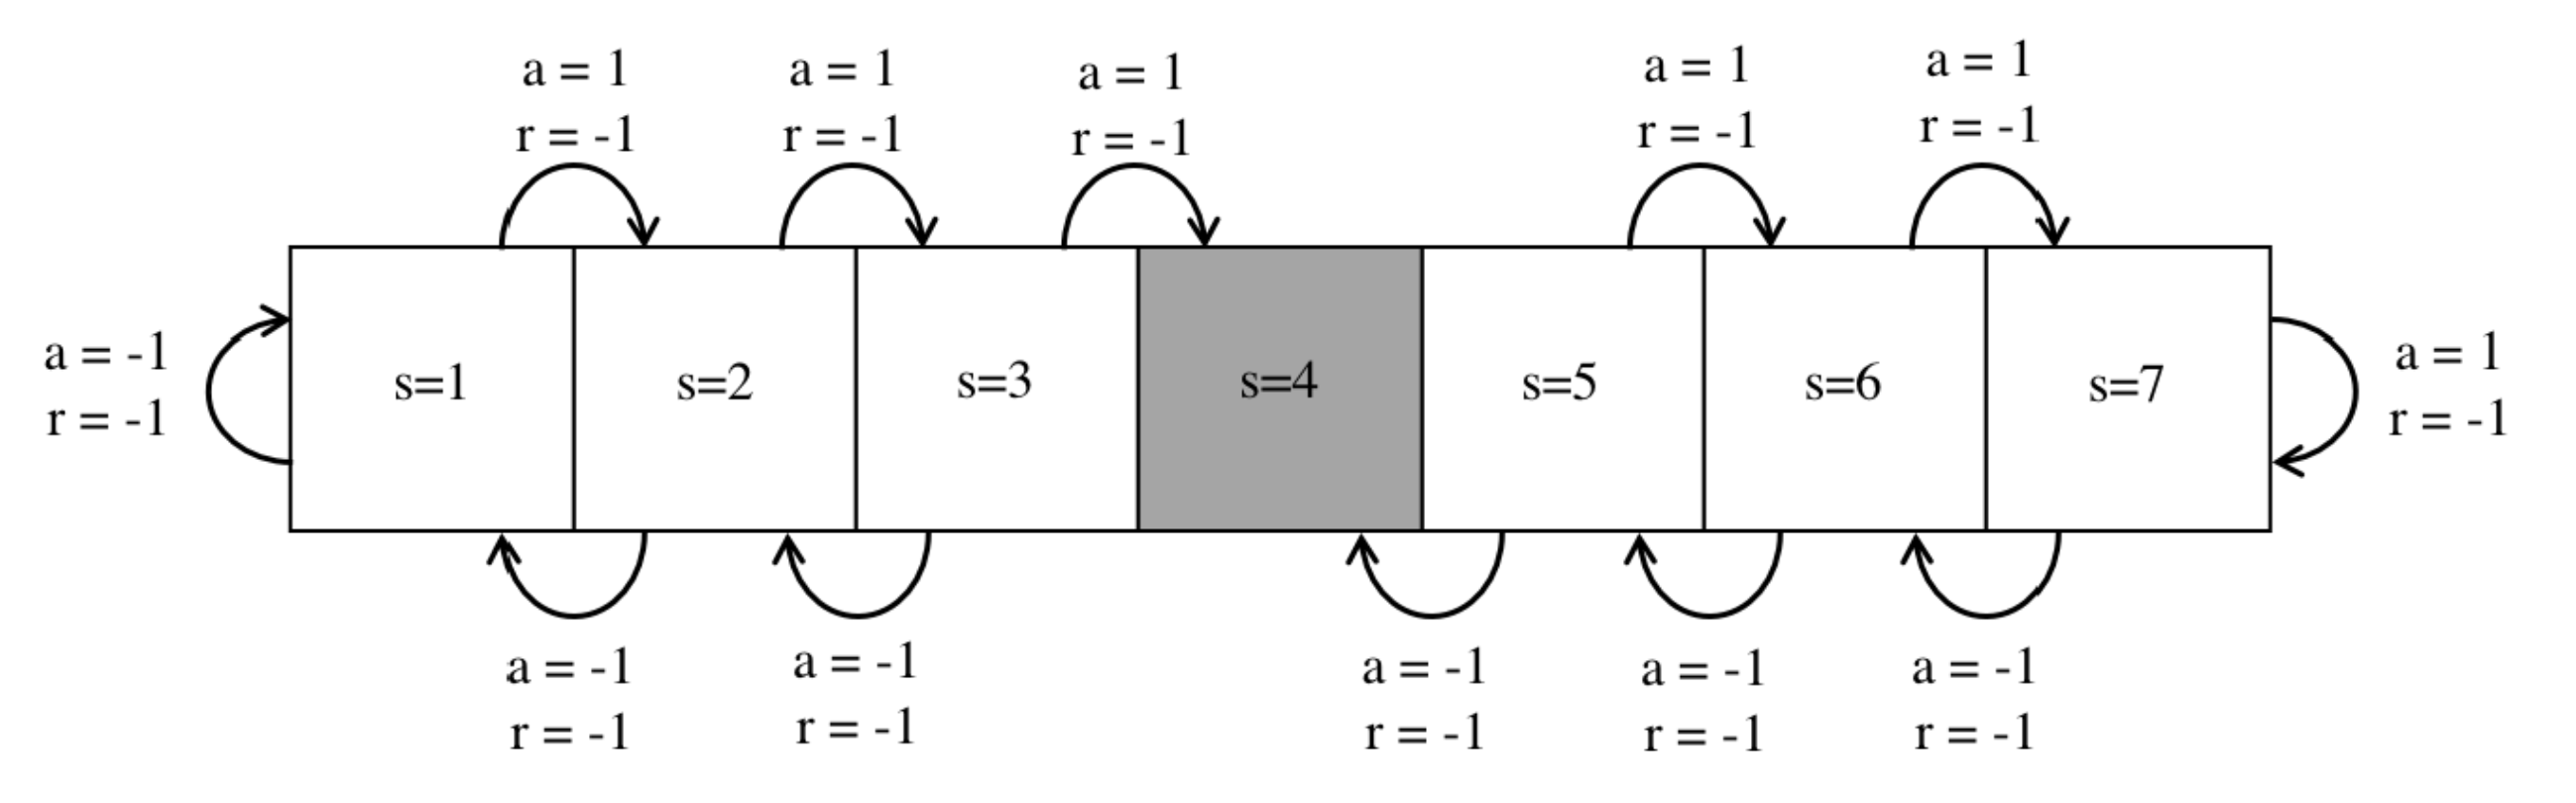
\includegraphics[width=0.9\linewidth]{images/p3.png}
    \caption{MDP procedure with seven states.}
    \label{figp3}
\end{figure}
By inspection, we see that $V^{*}=-|s-4|$
\begin{enumerate}[a.]
    \item We would like to perform tabular Q-learning on this chain MDP. Suppose we observe the following 4 step trajectory (in the form (state, action, reward)):
    $$
    (3,-1,-1),(2,1,-1),(3,1,-1),(4,1,0)
    $$
    Suppose we initialize all Q values to 0 . Use the tabular Q-learning update to give updated values for
    $$
    Q(3,-1), Q(2,1), Q(3,1)
    $$
    assuming we process the trajectory in the order given from left to right. Use the learning rate $\alpha=1 / 2$.

    \text { [Hints: Using } $\left.Q(s, a) \leftarrow Q(s, a)+\alpha\left(r+\gamma \max _{a^{\prime} \in\{1,-1\}} Q\left(s^{\prime}, a^{\prime}\right)-Q(s, a)\right)\right]$
\end{enumerate}

Now, we are interested in performing linear function approximation in conjunction with Qlearning. In particular, we have a weight vector $w=\left[w_{0}, w_{1}, w_{2}\right]^{T} \in \mathbb{R}^{3}$. Given some state $s$ and
action $a \in\{-1,1\}$, the featurization of this state, action pair is: $[s, a, 1]^{T}$. To approximate the $\mathrm{Q}$ -
values, we compute
$$
\hat{q}(s, a ; w)=\left[w_{0}, w_{1}, w_{2}\right][s, a, 1]^{T}=w_{0} * s+w_{1} * a+w_{2}
$$
Given the parameters $w$ and a single sample $\left(s, a, r, s^{\prime}\right)$. The loss function we will minimize is
$$
J(w)=\left(r+\gamma \max _{a^{\prime}} \hat{q}\left(s^{\prime}, a^{\prime} ; w^{-}\right)-\hat{q}(s, a ; w)\right)^{2}
$$
where $\hat{q}\left(s^{\prime}, a^{\prime} ; w^{-}\right)$ is a target network parameterized by fixed weights $w^{-}$.
\begin{enumerate}[a.]
    \setcounter{enumi}{1} 
    \item Suppose we currently have a weight vectors $w=[-1,1,1]^{T}$ and $w^{-}=[1,-1,-2]^{T}$, and we observe a sample $\left(s=2, a=-1, r=-1, s^{\prime}=1\right)$.
    Perform a single gradient update to the parameters $w$ given this sample. Use the learning rate $\alpha=1 / 4 .$ Write out the gradient $\nabla_{w} J(w)$ as well as the new parameters $w^{\prime}$.
    \item The optimal Q function $Q^{*}(s, a)$ is exactly representable by some neural
    network architecture $N$. Suppose we perform Q-learning on this MDP using the architecture $N$ to represent the Q-values. Suppose we randomly initialize the weights of a neural net with architecture $N$ and collect infinitely many samples using an exploration strategy that is greedy in the limit of infinite exploration (GLIE). Are we guaranteed to converge to the optimal $\mathrm{Q}$ function $Q^{*}(s, a) ?$ Explain it.
\end{enumerate}

\vspace{4pt}
\textbf{\large{Solution}}

\vspace{4pt}
\textbf{Subproblem(a)}

Given $\left(s, a, r, s^{\prime}\right)$, we use the update equation:
$$
Q(s, a) \leftarrow Q(s, a)+\alpha\left(r+\gamma \max _{a^{\prime} \in\{-1,1\}} Q\left(s^{\prime}, a^{\prime}\right)-Q(s, a)\right)
$$

Using this equation with $\alpha=\frac{1}{2}, \gamma=\frac{1}{3}$, we have:
\begin{equation}\nonumber
    \begin{split}
        Q(3,-1) \leftarrow 0+\frac{1}{2}\left(-1+\frac{1}{3}\max _{a^{\prime}} Q\left(2, a^{\prime}\right)\right)&=\frac{1}{2}(-1+0)=-\frac{1}{2} \\
        Q(2,1) \leftarrow 0+\frac{1}{2}\left(-1+\frac{1}{3}\max _{a^{\prime}} Q\left(3, a^{\prime}\right)\right) &=\frac{1}{2}(-1+0)=-\frac{1}{2} \\
        Q(3,1) \leftarrow 0+\frac{1}{2}\left(-1+\frac{1}{3}\max _{a^{\prime}} Q\left(4, a^{\prime}\right)\right) &=\frac{1}{2}(-1+0)=-\frac{1}{2}
    \end{split}
\end{equation}

\vspace{4pt}
\textbf{Subproblem(b)}

We have $\nabla_{w} J(w)$ as follow
$$
\begin{aligned}
\nabla_{w} J(w) &=-2\left(r+\gamma \max _{a^{\prime}} \hat{q}\left(s^{\prime}, a^{\prime} ; w^{-}\right)-\hat{q}(s, a ; w)\right) \nabla_{w} \hat{q}(s, a ; w) \\
&=-2\left(r+\frac{1}{3}\max _{a^{\prime}}\left(w^{-}\right)^{T}\left[\begin{array}{c}
s^{\prime} \\
a^{\prime} \\
1
\end{array}\right]-w^{T}\left[\begin{array}{l}
s \\
a \\
1
\end{array}\right]\right)\left[\begin{array}{l}
s \\
a \\
1
\end{array}\right]
\end{aligned}
$$
Using this, the parameter update with a single sample $\left(s, a, r, s^{\prime}\right)$ is:
$$
\begin{aligned}
w^{\prime} & \leftarrow w-\alpha \nabla_{w} J(w) \\
&=w+\frac{1}{2}\left(r+\frac{1}{3}\max _{a^{\prime}}\left(w^{-}\right)^{T}\left[\begin{array}{c}
s^{\prime} \\
a^{\prime} \\
1
\end{array}\right]-w^{T}\left[\begin{array}{l}
s \\
a \\
1
\end{array}\right]\right)\left[\begin{array}{l}
s \\
a \\
1
\end{array}\right]
\end{aligned}
$$
Using the sample $(2,-1,-1,1)$ and the particular values of $w$ and $w^{-}$ yields:
$$
\begin{aligned}
w^{\prime} & \leftarrow\left[\begin{array}{c}
-1 \\
1 \\
1
\end{array}\right]+\frac{1}{2}\left(-1+\frac{1}{3}\max _{a^{\prime}}\left[\begin{array}{c}
1 \\
-1 \\
-2
\end{array}\right]^{T}\left[\begin{array}{l}
1 \\
a^{\prime} \\
1
\end{array}\right]-\left[\begin{array}{c}
-1 \\
1 \\
1
\end{array}\right]^{T}\left[\begin{array}{c}
2 \\
-1 \\
1
\end{array}\right]\right)\left[\begin{array}{c}
2 \\
-1 \\
1
\end{array}\right] \\
&=\left[\begin{array}{c}
-1 \\
1 \\
1
\end{array}\right]+\frac{1}{2}\left(-1+\frac{1}{3}\max _{a^{\prime}}\left(1-a^{\prime}-2\right)-(-2-1+1)\right)\left[\begin{array}{c}
2 \\
-1 \\
1
\end{array}\right] \\
&=\left[\begin{array}{c}
-1 \\
1 \\
1
\end{array}\right]+\frac{1}{2}\left[\begin{array}{c}
2 \\
-1 \\
1
\end{array}\right] \\
&=\left[\begin{array}{c}
0 \\
1 / 2 \\
3 / 2
\end{array}\right]
\end{aligned}
$$

\vspace{4pt}
\textbf{Subproblem(c)}

Because this method of Q-learning involves function approximation, bootstrapping, and off-policy training, we are not guaranteed to converge to anything, which includes no guarantee of converging to the optimal Q function.
\end{homeworkProblem}

\begin{homeworkProblem}

\vspace{4pt}
\textbf{\large{Solution}}

\vspace{4pt}
\textbf{Subproblem(a)}

The codes please see the file \texttt{CIFAR\_A2.ipynb}.

\vspace{4pt}

We set \texttt{batch\_size=16}, and \texttt{epoch=20}, we can derive the training curve and test accuracy curve as Figure \ref{tr1}. As we can see, the test accuracy is about 65\% after 20 epochs.
\begin{figure}[H]
    \centering
    \subfigure[The training curve]{\label{}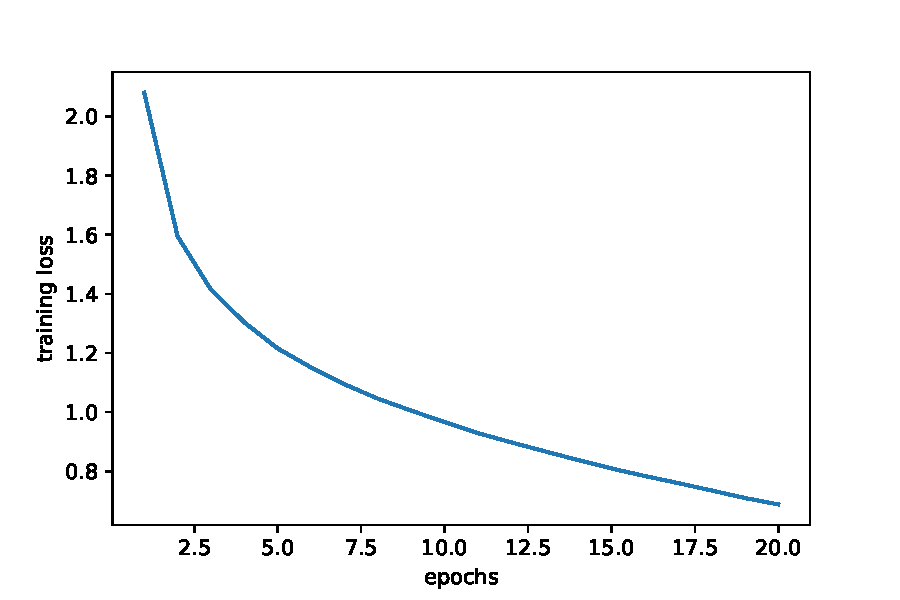
\includegraphics[width=0.47\linewidth]{images/loss1}}
    \quad
    \subfigure[The test accuracy curve]{\label{}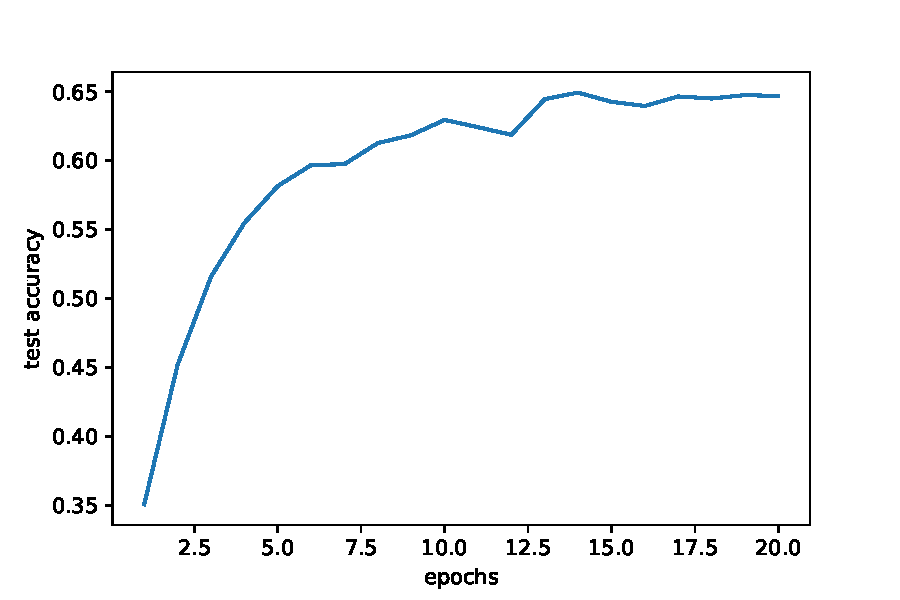
\includegraphics[width=0.47\linewidth]{images/accuracy1}}
    \caption{The plot of the training curve and test accuracy curve}
    \label{tr1}
\end{figure}
\vspace{4pt}
Then, we can visualize the filters learned in the first convolutional layer as Figure \ref{filter}. We do normalization to the weights in order to make the range of 
the weights in $\left[0,1\right]$.
\begin{figure}[!htbp]
    \centering
    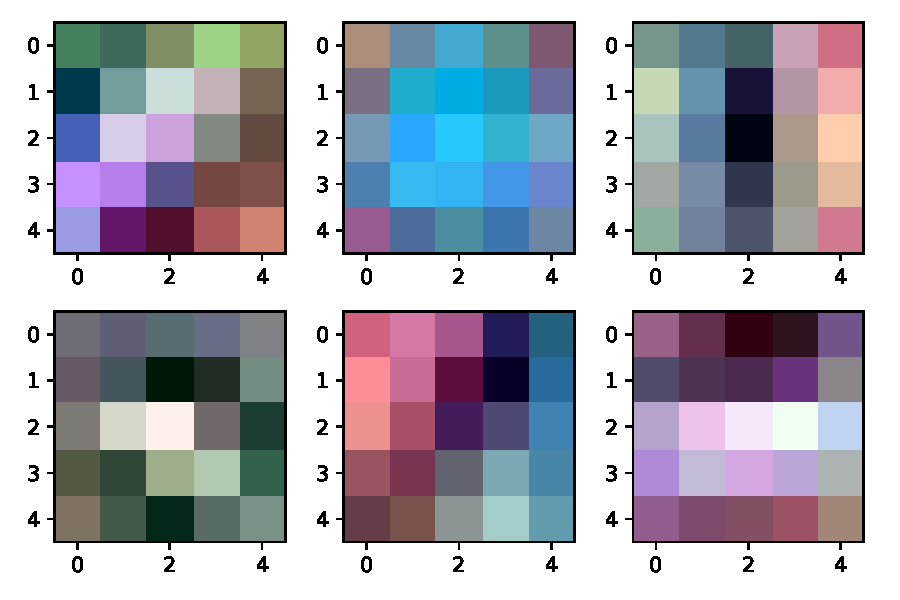
\includegraphics[width=0.8\linewidth]{images/vis}
    \caption{The filters learned in the first convolutional layer}
    \label{filter}
\end{figure}

\vspace{4pt}
\textbf{Subproblem(b)}

$\bullet$ We prove $\operatorname{Var}\left[y_{l}\right]=n_{l} \operatorname{Var}\left[w_{l}\right] \operatorname{E}\left[x_{l}^{2}\right]$ as follow
\begin{equation}
    \begin{split}
        \operatorname{Var}\left[y_{l}\right]&=\operatorname{Var}\left[\boldsymbol{W}_{l,i}\cdot\boldsymbol{x}_l\right]\\
        &=n_l\cdot \operatorname{Var}\left[w_l\cdot x_l\right]\\
        &=n_l\cdot \left(\operatorname{E}\left[\left(w_l\cdot x_l\right)^2\right]-\left(\operatorname{E}\left[w_l\cdot x_l\right]\right)^2\right)\\
        &=n_l\cdot \left(\operatorname{E}\left[\left(w_l\cdot x_l\right)^2\right]-\left(\operatorname{E}\left[w_l\right]\cdot \operatorname{E}\left[x_l\right]\right)^2\right)\\
        &=n_l\cdot \operatorname{E}\left[\left(w_l\cdot x_l\right)^2\right]\\
        &=n_l\cdot \operatorname{E}\left[w_l^2\right]\cdot\operatorname{E}\left[ x_l^2\right]\\
        &=n_l\cdot \operatorname{Var}\left[w_l\right]\cdot\operatorname{E}\left[ x_l^2\right]\\
    \end{split}
\end{equation}
$\bullet$ We prove $\operatorname{E}\left[x_{l}^{2}\right]=\frac{1}{2} \operatorname{Var}\left[y_{l-1}\right]$ as follow. If we let $w_{l-1}$ have a symmetric distribution around zero and $b_{l-1}=0$, then $y_{l-1}$ has zero mean and has a symmetric distribution around zero. 
We let $P(x)$ to denote the cdf of $x_l$, $p(x)$ to denote the pdf of $x_l$, and $Q(y)$ to denote the cdf of $y_{l-1}$, $q(y)$ to denote the pdf of $y_{l-1}$. Because the activation function $f$ is ReLu, so that we have
\begin{equation}
    \begin{split}
        &P\left(x\right)=
        \begin{cases}
            0&x<0\\
            \frac{1}{2}&x = 0\\
            Q\left(x\right)&x > 0\\
        \end{cases}\\
        \\
        &p\left(x\right)=q\left(x\right)\quad \left(x>0\right)
    \end{split}
\end{equation}
Then, we can have
\begin{equation}
    \label{eq12}
    \begin{split}
        \operatorname{E}\left[x_l^2\right]&=\int_{-\infty}^{+\infty}x_l^2\cdot p\left(x_l\right)dx_l\\
        &=0^2\cdot\frac{1}{2}+\int_{0}^{+\infty}x_l^2\cdot p\left(x_l\right)dx_l\\
        &=\int_{0}^{+\infty}x_l^2\cdot q\left(x_l\right)dx_l\\
    \end{split}
\end{equation}
We can also have
\begin{equation}
    \label{eq13}
    \begin{split}
        \frac{1}{2} \operatorname{Var}\left[y_{l-1}\right]&=\frac{1}{2} \operatorname{E}\left(y_{l-1}^2\right)\\
        &=\frac{1}{2}\int_{-\infty}^{+\infty}y_{l-1}^2 q\left(y\right)dy\\
        &=\frac{1}{2}\cdot 2 \int_{0}^{+\infty}y_{l-1}^2 q\left(y\right)dy\\
        &=\int_{0}^{+\infty}y_{l-1}^2 q\left(y\right)dy\\
    \end{split}
\end{equation}
By combination of equation \ref{eq12} and \ref{eq13}, we can see that $\operatorname{E}\left[x_{l}^{2}\right]=\frac{1}{2} \operatorname{Var}\left[y_{l-1}\right]$. Thus, we finished the proof.

\vspace{4pt}
Then, we use the weight initialization strategy, and get the  training curve and test accuracy curve as Figure \ref{kaiming}. As we can see, the test accuracy is still about 65\% after 20 epochs, which seems no improvement. 
The reason is maybe that the original initialization is good enough.
\begin{figure}[H]
    \centering
    \subfigure[The training curve]{\label{}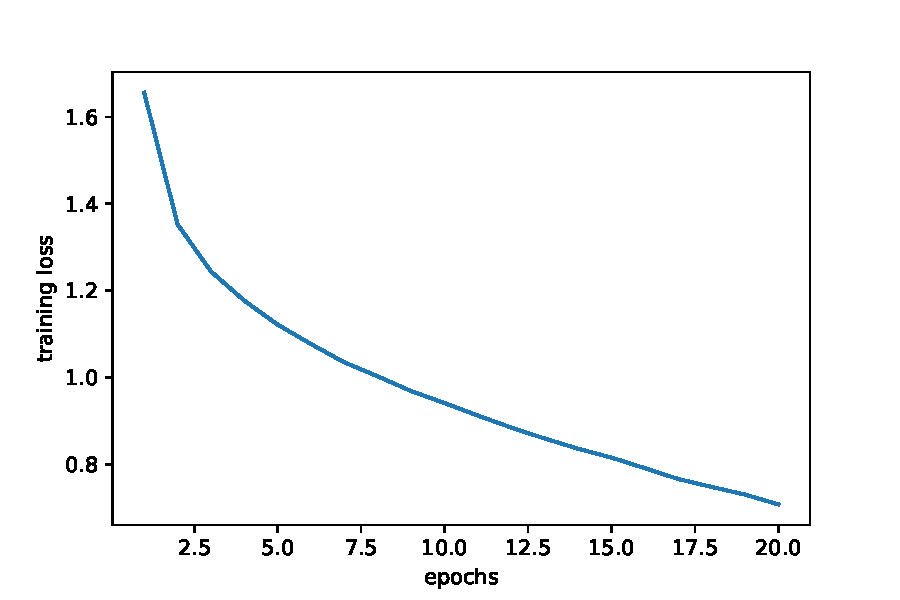
\includegraphics[width=0.47\linewidth]{images/loss_kaiming}}
    \quad
    \subfigure[The test accuracy curve]{\label{}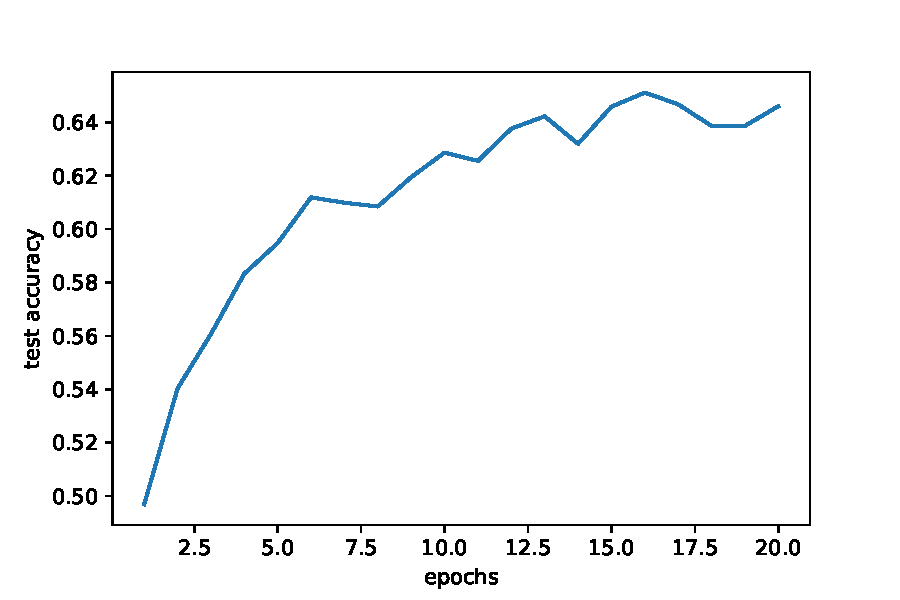
\includegraphics[width=0.47\linewidth]{images/accuracy_kaiming}}
    \caption{The plot of the training curve and test accuracy curve with kaiming initialization}
    \label{kaiming}
\end{figure}
\vspace{4pt}
\textbf{Subproblem(c)}

By using batch normalization, we can get the  training curve and test accuracy curve as Figure \ref{BN}. As we can see, the test accuracy reaches 66\% after 20 epochs. Besides, the trend seems to 
increase continuously, so we believe that the test accuracy will be higher after more epochs. Thus, the batch normalization is really helpful.
\begin{figure}[H]
    \centering
    \subfigure[The training curve]{\label{}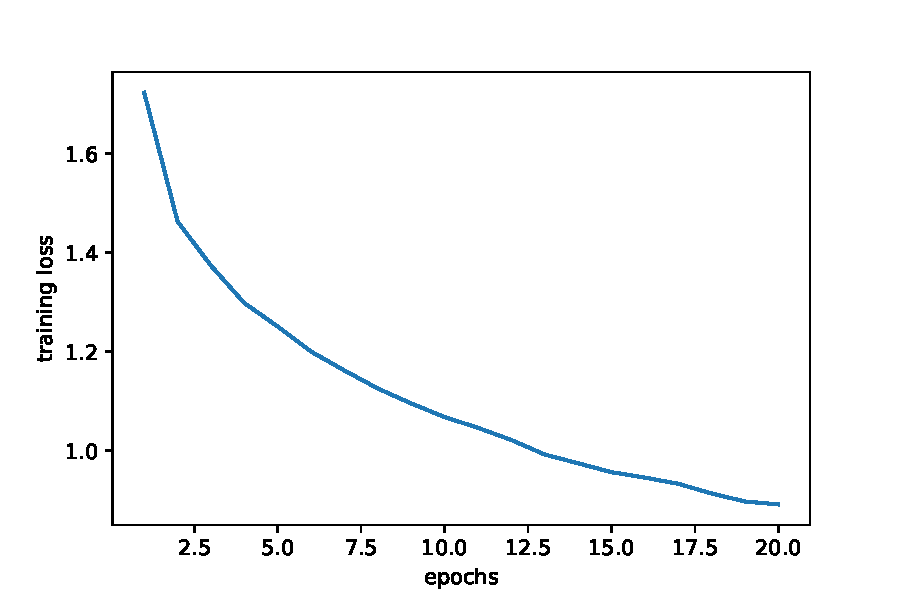
\includegraphics[width=0.47\linewidth]{images/loss_BN}}
    \quad
    \subfigure[The test accuracy curve]{\label{}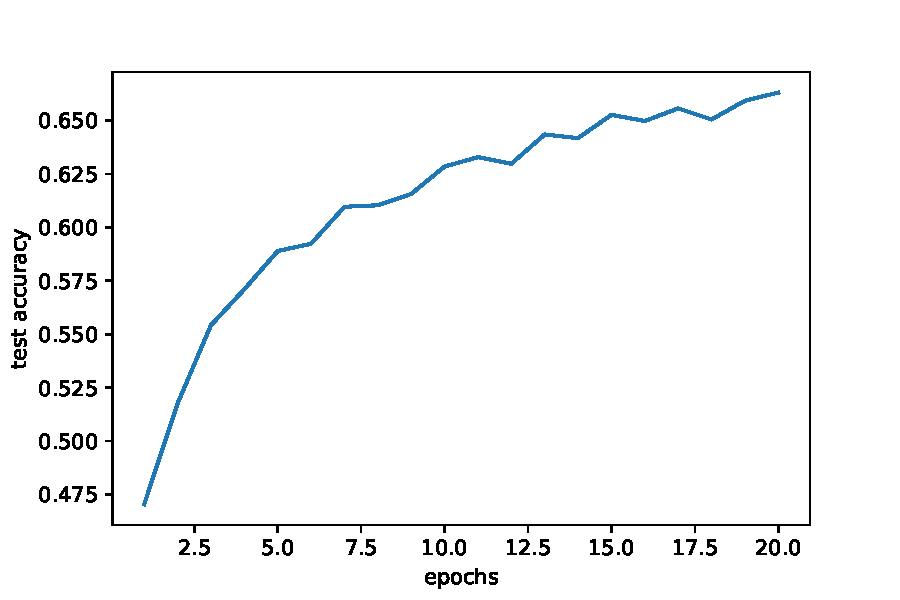
\includegraphics[width=0.47\linewidth]{images/accuracy_BN}}
    \caption{The plot of the training curve and test accuracy curve with kaiming initialization and batch normalization}
    \label{BN}
\end{figure}

\vspace{4pt}
\textbf{Subproblem(d)}

We try to ues Adam as the optimizer, and we can get the training curve and test accuracy curve as Figure \ref{adam}. As we can see, the test accuracy reaches 69\% after 20 epochs, which is higher than before. Thus, we can see Adam optimizer if very helpful.
\begin{figure}[H]
    \centering
    \subfigure[The training curve]{\label{}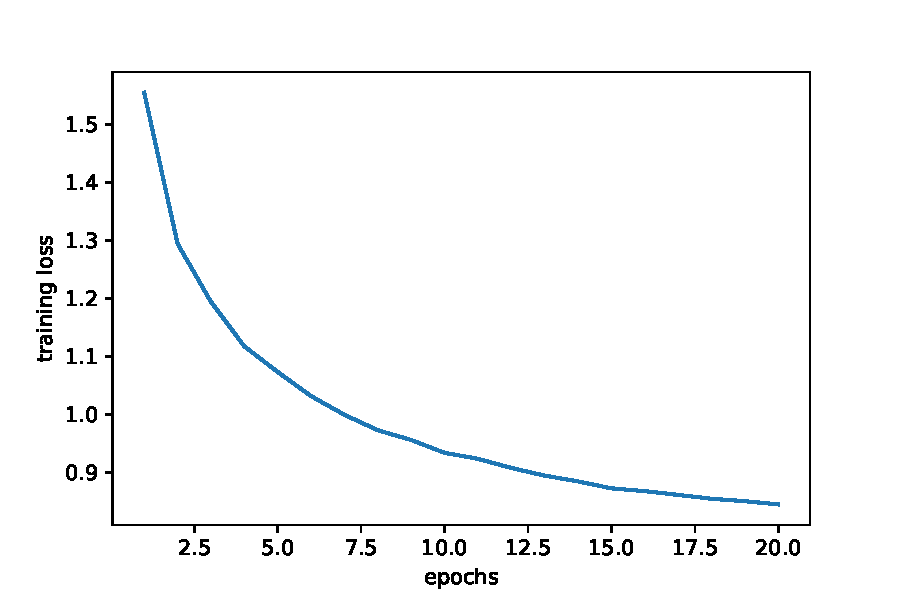
\includegraphics[width=0.47\linewidth]{images/loss_Adam}}
    \quad
    \subfigure[The test accuracy curve]{\label{}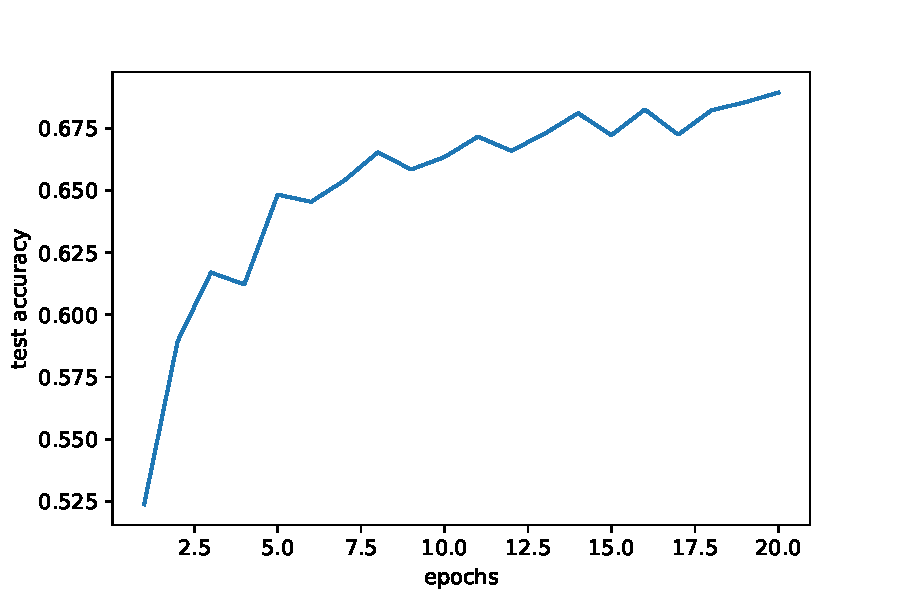
\includegraphics[width=0.47\linewidth]{images/accuracy_Adam}}
    \caption{The plot of the training curve and test accuracy curve with kaiming initialization and batch normalization, and Adam optimizer}
    \label{adam}
\end{figure}
\end{homeworkProblem}
\end{document}

